
\documentclass[a4paper,12pt,oneside]{scrreprt}
\usepackage[latin1]{inputenc}
\usepackage[T1]{fontenc}
\usepackage{ae,aecompl}
\usepackage[english]{babel}
\usepackage{amsmath}
\usepackage{amssymb}
\usepackage{amsfonts}
\usepackage{amsthm}
\usepackage{graphicx}
\usepackage{wrapfig}
\usepackage{ulem}
\usepackage{cancel}
\usepackage{float}
\usepackage{color}
%\usepackage{titlesec}
\usepackage{geometry}
\geometry{verbose,a4paper,tmargin=25mm,bmargin=25mm,lmargin=15mm,rmargin=16mm}

\usepackage{tabularx}
\usepackage{booktabs}
\usepackage{paralist}
\usepackage{textcomp}
\usepackage[official]{eurosym}

\renewcommand{\rmdefault}{phv}
\renewcommand{\sfdefault}{phv}

% for splitting page into many pages vertically
\usepackage{paracol}
\usepackage{url}

% our OWN imports for our use
\usepackage{listings}
\lstdefinestyle{ourJavaStyle}{
	language=Java,
	numbers=left,
	%numbersep=8pt,
	stepnumber=1,
	tabsize=2,
	showspaces=false,
	showstringspaces=false,
	basicstyle=\ttfamily\scriptsize,
	keywordstyle=\color{blue}\ttfamily,
	stringstyle=\color{red}\ttfamily,
	commentstyle=\color{green}\ttfamily,
	breaklines=true
}

\newcommand*{\sourcepath}{../code/src/main/java}
\newcommand*{\testpath}{../code/src/test/java}

\setcounter{chapter}{5} % Aktuelles Assigment

% naming convention for LaTeX report
% subsub/sub/section naming: 
%		chapter: number (unchanged)
%		section: number (unchanged)
%		subsect: letter
%		subsubs: letter
\renewcommand{\thesubsection}{\thesection.\alph{subsection}}
\setcounter{secnumdepth}{3}
\renewcommand{\thesubsubsection}{\thesubsection.\alph{subsubsection}}

%\usepackage[magyar]{babel}

\makeatletter
\expandafter\let\csname active@char\string?\endcsname\relax
\expandafter\let\csname active@char\string!\endcsname\relax
\expandafter\let\csname active@char\string:\endcsname\relax


\initiate@active@char{?}
\initiate@active@char{!}
\initiate@active@char{:}
\makeatother

\begin{document}
	
	\begin{tabular}{ccc}
		\begin{large} \textbf{Prof. Lichter} \end{large} &
		
		\begin{minipage}[H]{3.5cm}
			\centering
			\begin{large} OOSC \end{large} \\
			\begin{large} WS 2019/2020 \end{large}
		\end{minipage} &
		
		\begin{minipage}[H]{4cm}
			
\includegraphics[keepaspectratio,width=\textwidth,angle=0]{images/swc.png}
		\end{minipage} \\
		Andreas Steffens, Konrad F\"ogen &  &  \\
		& \begin{huge} \textbf{Submission 5} \end{huge}&  \\
		& oosc@swc.rwth-aachen.de &  \\
		& & \\
		% Hier drunter muessen die Daten noch angepasst werden
		Issued: 16.12.2019 &
		Submission: 06.01.2020 &
		Discussion: 09.01.2020 \\
	\end{tabular}
	\newline \newline \newline
	\begin{center}
		Submitted by Group 10
		
		\begin{tabular}{ll}
			Dominik Bittner, & 369202 \\
			Ulfet Cetin, & 391819\\
			Mubasher Chaudhary (Group 02), & 391871 \\
			Philipp Hochmann, & 356148 \\
			Anar Orujov, & 391825\\
			Ada Slupczynski, & 384147\\
			(sorted on lastname basis)
		\end{tabular}
	\end{center}

	
	% !TEX root = ../Group10_Assignment6_OOSC_2020.tex

\section{Frameworks}

\subsection{Actions Supported}

\begin{itemize}
	\item calculate flat size
	\begin{itemize}
		\item in the current state of SWCArchitect (that is implemented in the previous assignment), we have the 'import floorplan' function. Through that, we can get the information on the imported image, such as width and height.
		\item however, those features of width and height are abstract, they do not map to the real-world information without extra information. Due to this nature of those features, we can either:
		\begin{itemize}
			\item provide flat size in pixel$^{2}$ (e.g. height * width)
			\item we can ask for user intervention, that, at the import of floorplan, we can ask user to provide the dimensions of the flat, so we can map those real world values to the pixels. This would help us also in the other functionalities.
		\end{itemize}
		\item in the previous assignment, we have extended ImageTool to build our ImageImporter (for floorplan). This class' implementation can be used to implement this functionality of calculating flat size.
	\end{itemize}
	\bigskip
	
	\item occupied space of elements/free space
	\begin{itemize}
		\item similar to the 'calculate flat size', we can either ask for user intervention for meter$^{2}$ calculation, or even better, ask for room size once. If we have such information, then we have what is the length of each pixel in horizontal and vertical directions. With such information, we can calculate the relative size of the furnitures too.
		\item in the same sense, we implemented furnitures by extending TextAreaFigure, and we can use this to implement the given functionality.
	\end{itemize}
	\bigskip
	
	\item validate constraints, e.g. "a room has at least three connected walls"
	\begin{itemize}
		\item in the previous assignment, we also implemented some of the constraints.\\
		Citing from our own previous assignment:
		
		\begin{addmargin}[4em]{0em}
			\textit{Wall, Door and Window are extending ImageFigure. Also, Door and Window are created by a special
				CreationTool named "CreateInWallElement". It checks that doors and windows are always placed on a
				wall. If not, it intercepts the call of the framework to mousePressed.}
		\end{addmargin}
		
		\item we can use this to enforce some of the constraints. For the rest of the constraints, we would use Template-Hook approach to enable user to add more constraint by coding, if a need is deemed necessary.
	\end{itemize}
	
	\item mass operations (resizing of multiple objects)
	\begin{itemize}
		\item multiple items can be chosen \& resized.\\
			In order to allow grouping, such as:
			\begin{itemize}
				\item only group certain kind of furniture (e.g. only chairs)
				\item group more than one kind of furniture (like the example in the previous assignment: table \& chair grouping)
			\end{itemize}
	
		\item for such flexibility, we would also use one of the Template-Hook approaches, so the user-generated furniture types are also allowed to be grouped without selecting them manually.
	\end{itemize}
\end{itemize}

\subsection{UI choice}

We would like to select the first of the provided UI dialogues. Thanks to the jHotDraw support of the menu implementation, it would allow for an easier and cleaner implementation of the inclusion of additional features. A drop-down added to the menu-bar would also allow for the users to already feel comfortable with functionality that is added in an intuitive way. We believe that the second UI could confuse potential users of our application with regards to the behaviour of the added functionality.

\subsection{Framework properties and patterns}
We would like to define this framework as a white-box framework, as it will be an extension of the jHotDraw framework. We would like to propose an implementation that would allow the usage of elements such as Figures. For that to work nicely, we would like to propose the following patterns to provide support of our implementation:

\subsubsection{Calculate flat size}
For the calculation of the flat area, we would like to propose the usage of \textbf{Singleton Pattern}. We would like to additionally ask the user after they upload a background image to provide the width and height of the flat. Those could then be mapped onto the amount of pixels in width and height respectively to be able to approximate the size of each of the elements. This means that the flat size would be not only an accurate measure, but also easily accessible by all components that need it.

\subsubsection{Occupied space of elements/free space}
The calculation of the occupied space/free space would also follow a similar set of steps as the flat size, but due to various object types usage, we would like to use the \textbf{Template Method Pattern}. This would allow us to provide an abstract structure containing general methods of concepts, which we could then be made more concrete in the respective classes, which define the calculation of specific object types. The calculation of the occupied space would then simply be made by addition of the results of the helper classes. One could then obtain the free space based on the subtraction between the flat size and the above mentioned addition result.

\subsubsection{Validate constraints}
For the validation of constraints we would like to propose the \textbf{1:n Connection meta-pattern} with \textbf{Observer pattern}. Not only would we then be able to define constraints for various types of objects, but also provide a quick response to the changes made in the UI by the user. This is very important in the constraint validation. As we have various object types and various constraints that are relevant to them, the 1:n Connection seems a relatively obvious choice.
The notify in the ConstraintHolder would then be responsible for keeping track of all elements, which are managed in terms of a specific type of constraints and notifying all relevant observers if a constraint violation has been detected. ConstraintHolder contains also a list of all constraints to help in the notify process.

\subsubsection{Mass operations}
We would like to propose the usage of event listeners in each of the objects. When the user would like to for example resize all chairs in the image, they would have to emit chair resize event, which would trigger all relevant chairs to update their sizing accordingly.


\subsection{UML Diagrams}

\subsubsection{Area Calculations}

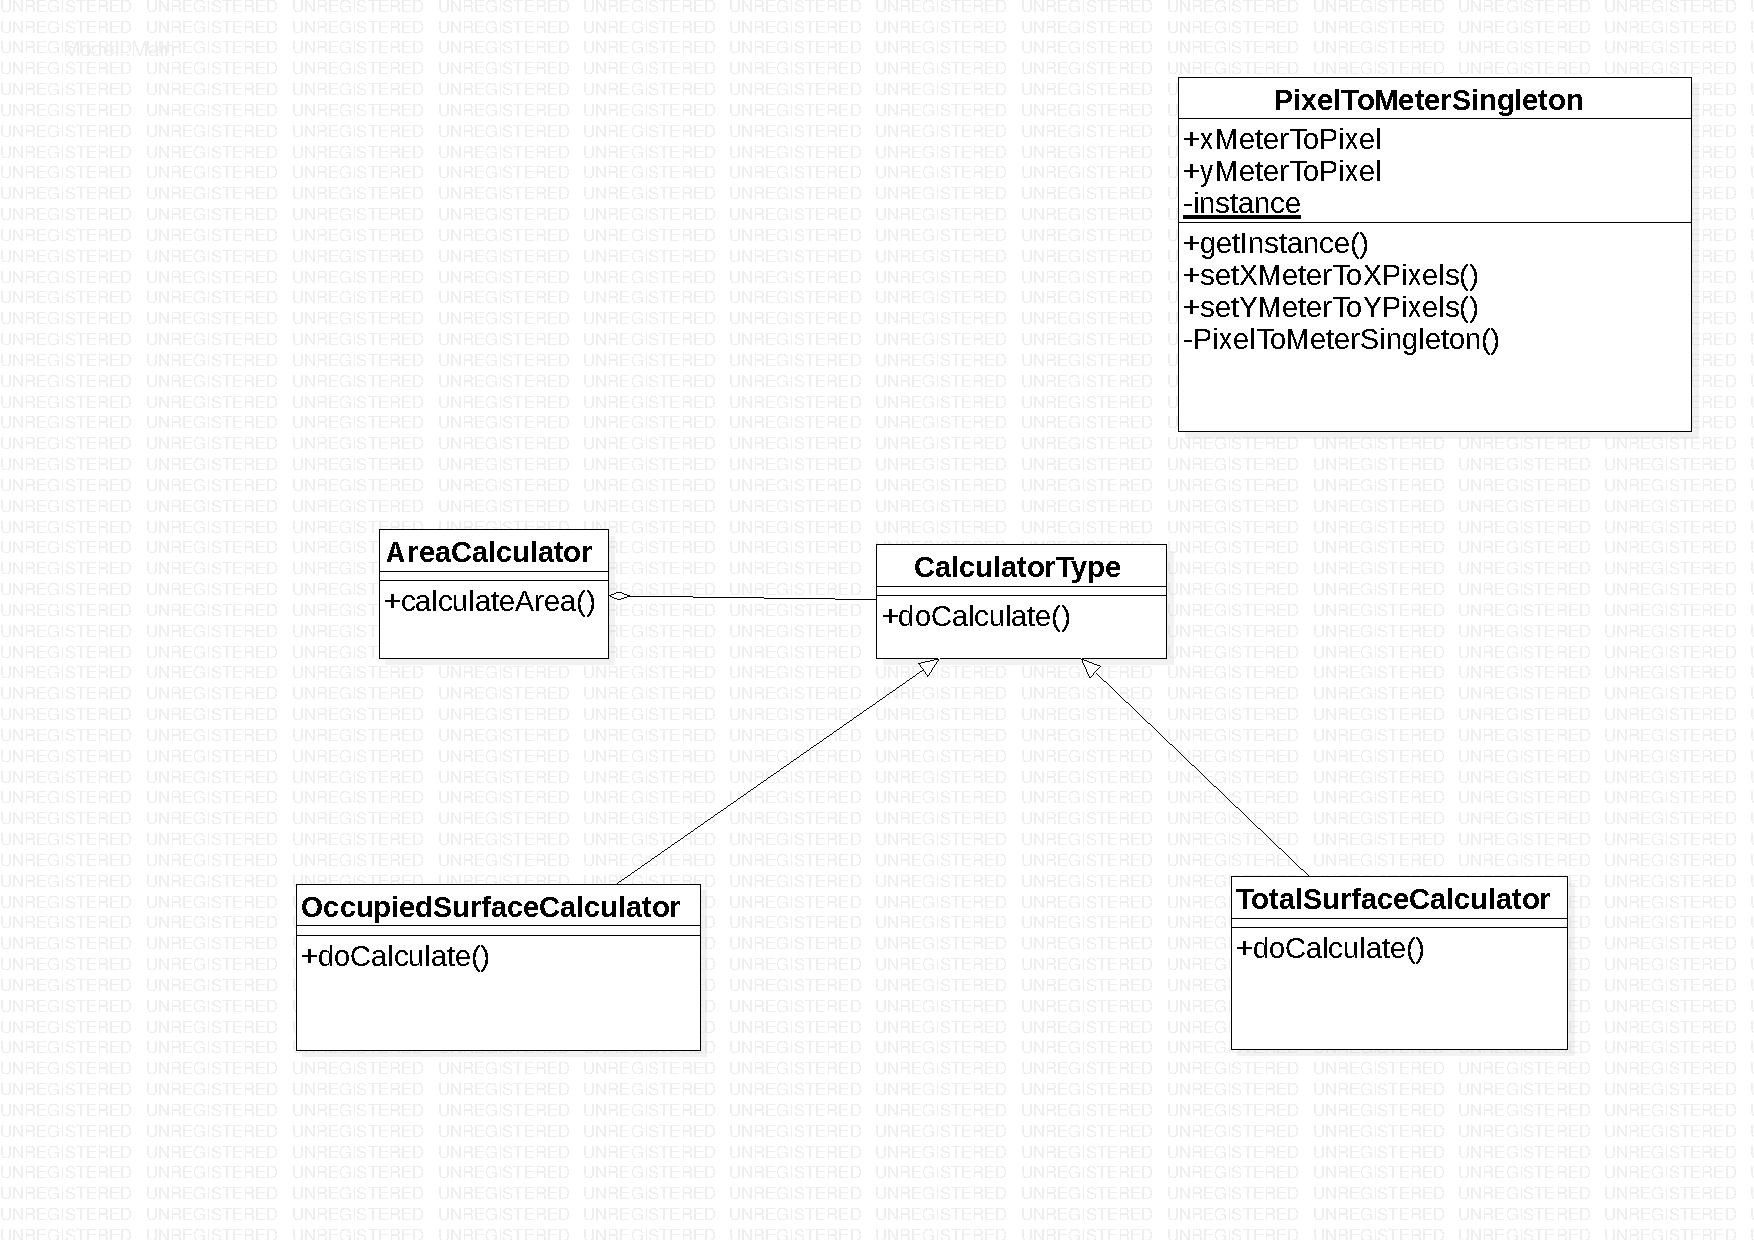
\includegraphics[width=\textwidth]{../uml/area}

\subsubsection{Constraint Validation}

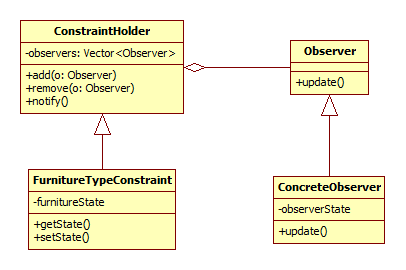
\includegraphics[width=\textwidth]{../uml/constraint.png}

	
	\section{Components}

After making clear that there is a timeframe for successful completion of the tasks, and that coming earlier (a.k.a rushing) would not grant a user any benefit, we updated our storyboard as follows:

\subsection{SketchImporter}
	\begin{description}
		\item[Decision] \hfill \\ Bad suggestion
		\item[Justification] \hfill \\ It is too specific and hence not reusable. It should be ImageImporter, which would give user a choice whether it is a furniture piece or a floor plan.
		\item[Interfaces] \hfill \\ -
		\item[Interactions with other components] \hfill \\ -
		\item[Included classes or entities] \hfill \\ -
		\item[Integration with JHotDraw] \hfill \\ -
	\end{description}

\subsection{FlatModeler}
	\begin{description}
		\item[Decision] \hfill \\ Bad suggestion
		\item[Justification] \hfill \\ It is very general and would basically contain the entire functionality, whereas components are supposed to be smaller and limited to a certain type of functionality (like WallModeler).
		\item[Interfaces] \hfill \\ -
		\item[Interactions with other components] \hfill \\ -
		\item[Included classes or entities] \hfill \\ -
		\item[Integration with JHotDraw] \hfill \\ -
	\end{description}

\subsection{ImageExporter}
	\begin{description}
		\item[Decision] \hfill \\ Good suggestion
		\item[Justification] \hfill \\ It is small functionality part in a very defined context. One knows it is used for exporting images.
		\item[Interfaces] \hfill \\ public URIChooser createExportChooser(Application a, @Nullable View v)
		\item[Interactions with other components] \hfill \\ ExportFileAction
		\item[Included classes or entities] \hfill \\ URIChooser, Application, View
		\item[Integration with JHotDraw] \hfill \\ A button on a toolbar.
	\end{description}

\subsection{WebPublisher}
	\begin{description}
		\item[Decision] \hfill \\ Good component
		\item[Justification] \hfill \\ Again, the usage of this component is clear and understandable from the name.
		\item[Interfaces] \hfill \\ publishPlan(image, author)
		\item[Interactions with other components] \hfill \\ -
		\item[Included classes or entities] \hfill \\ Some communication classes, also some conversion classes needed.
		\item[Integration with JHotDraw] \hfill \\ A button on a toolbar.
	\end{description}

\subsection{FurnitureFactory}
	\begin{description}
		\item[Decision] \hfill \\ Bad suggestion
		\item[Justification] \hfill \\ Dependant on the context and hence not reusable.
		\item[Interfaces] \hfill \\ -
		\item[Interactions with other components] \hfill \\ -
		\item[Included classes or entities] \hfill \\ -
		\item[Integration with JHotDraw] \hfill \\ -
	\end{description}

\subsection{ChairTableGrouping}
	\begin{description}
		\item[Decision] \hfill \\ Bad suggestion
		\item[Justification] \hfill \\ If we want to group any other types, it is not reusable as it depends on the chair and the table type.
		\item[Interfaces] \hfill \\ -
		\item[Interactions with other components] \hfill \\ -
		\item[Included classes or entities] \hfill \\ -
		\item[Integration with JHotDraw] \hfill \\ -
	\end{description}

\subsection{ConstraintValidation}
	\begin{description}
		\item[Decision] \hfill \\ Bad suggestion
		\item[Justification] \hfill \\ Very general as there are different constraints for various types of furniture - one can fill the space under the table with something, which is not the case with a solid object like the drawer. Each object group should have its own constraint validation. Additionally, one should run the constraint validation after attempted placement of the object to avoid computation overhead.
		\item[Interfaces] \hfill \\ -
		\item[Interactions with other components] \hfill \\ -
		\item[Included classes or entities] \hfill \\ -
		\item[Integration with JHotDraw] \hfill \\ -
	\end{description}

Decide for each of the following suggestions if they are components and justify your
answer. In the case of a good component candidate extend the description with
Interfaces
Interactions with other components
Included classes or entities
Integration with JHotDraw

% \subsection{SketchImporter}
% This is a good choice for a component. It is a small part of the program, which could also be used in different drawing programs. Expect of the dependency to JHotDraw it has no further dependencies and therefore is well suited for an own component.

% In general this component should receive an image file and import this to the given drawing but the interface looks a bit different because of the implementation with JHotDraw: The component is implemented as a \textit{Tool} and is an extension of \textit{ImageTool}. But only the \textit{creationFinished} method is overwritten. The \textit{ImageTool} already provides a functionality to import an image to the drawing. With the extension this image is set to the background and positioned to the (0,0) point. As the \textit{ImageTool}, this component also requires an \textit{ImageFigure} as constructor parameter and interact directly to the current view of this JHotDraw application.

% \subsection{ImageExporter}
% The ImageExporter is not a good choice for a component. The exporting feature is a general feature for a drawing application and therefore it is more clever to integrate this to the framework directly. So it could be extended by different applications for different needs, for example different file formats to export.

% In JHotDraw is an exporter feature already implemented. It could be provided through the \textit{ExportFileAction}. In addition to this to hot spots have to be implemented: In the \textit{ApplicationModel} the method \textit{createExportChooser} have to be overwritten to show all available formats in the export dialog and the method \textit{write} in the \textit{View} have to be changed to save the drawing in the selected format.

	
	\section{Implementation}

\subsection{SketchImporter}

This component is implemented as a \textit{Tool} and is an extension of \textit{ImageTool}. But only the \textit{creationFinished} method is overwritten. The \textit{ImageTool} already provides a functionality to import an image to the drawing. With the extension this image is set to the background and positioned to the (0,0) point. As the \textit{ImageTool}, this component also requires an \textit{ImageFigure} as constructor parameter and interact directly to the current view of this JHotDraw application.

For the implementation of the SketchImporter component two classes were created: The \textit{BackgroundImageTool} and the \textit{ZeroPointMoveAction}. The second one is just a helper class which is used by the other to move the imported image to the "`zero point"' (0,0) and therefore extends the abstract \textit{MoveAction}.
The \textit{BackgroundImageTool} extends the \textit{ImageTool}-class provided by JHotDraw. The basic image import is already implemented there. The imported image is only moved to the right location and set as background. Therefore the \textit{DrawingView} has to be used, which could be accessed through the \textit{getView} method.

\begin{figure}[h]
    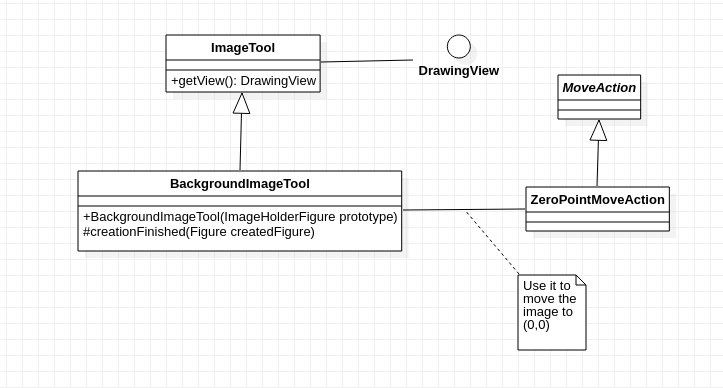
\includegraphics[keepaspectratio,width=\textwidth]{images/SketchImporter.png}
    \caption{SketchImporter Implementation}
\end{figure}

	
	\clearpage
\section{Use the SWCArchitect}

One can find all the following pictures in our submission archive.\\
Here are the usage snapshots of our SWCArchitect.

\begin{figure}[h]
	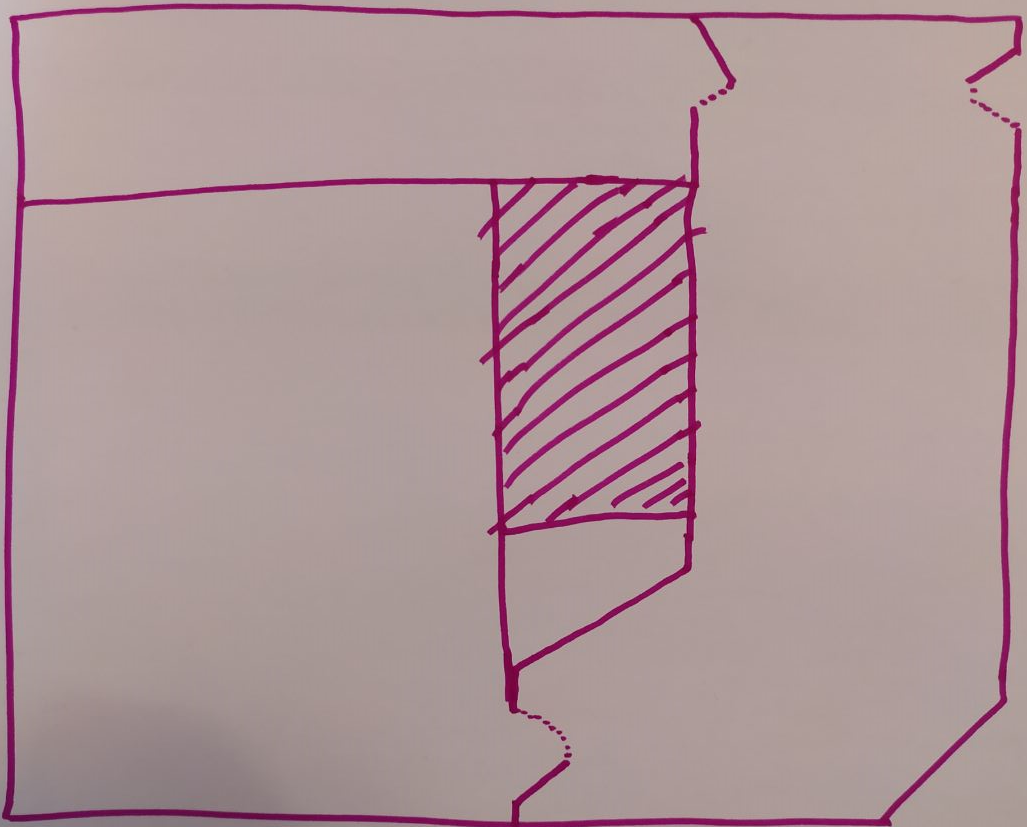
\includegraphics[keepaspectratio,width=\textwidth]{images/input.png}
	\caption{Hand-Drawn Floorplan}
\end{figure}

\begin{figure}[h]
	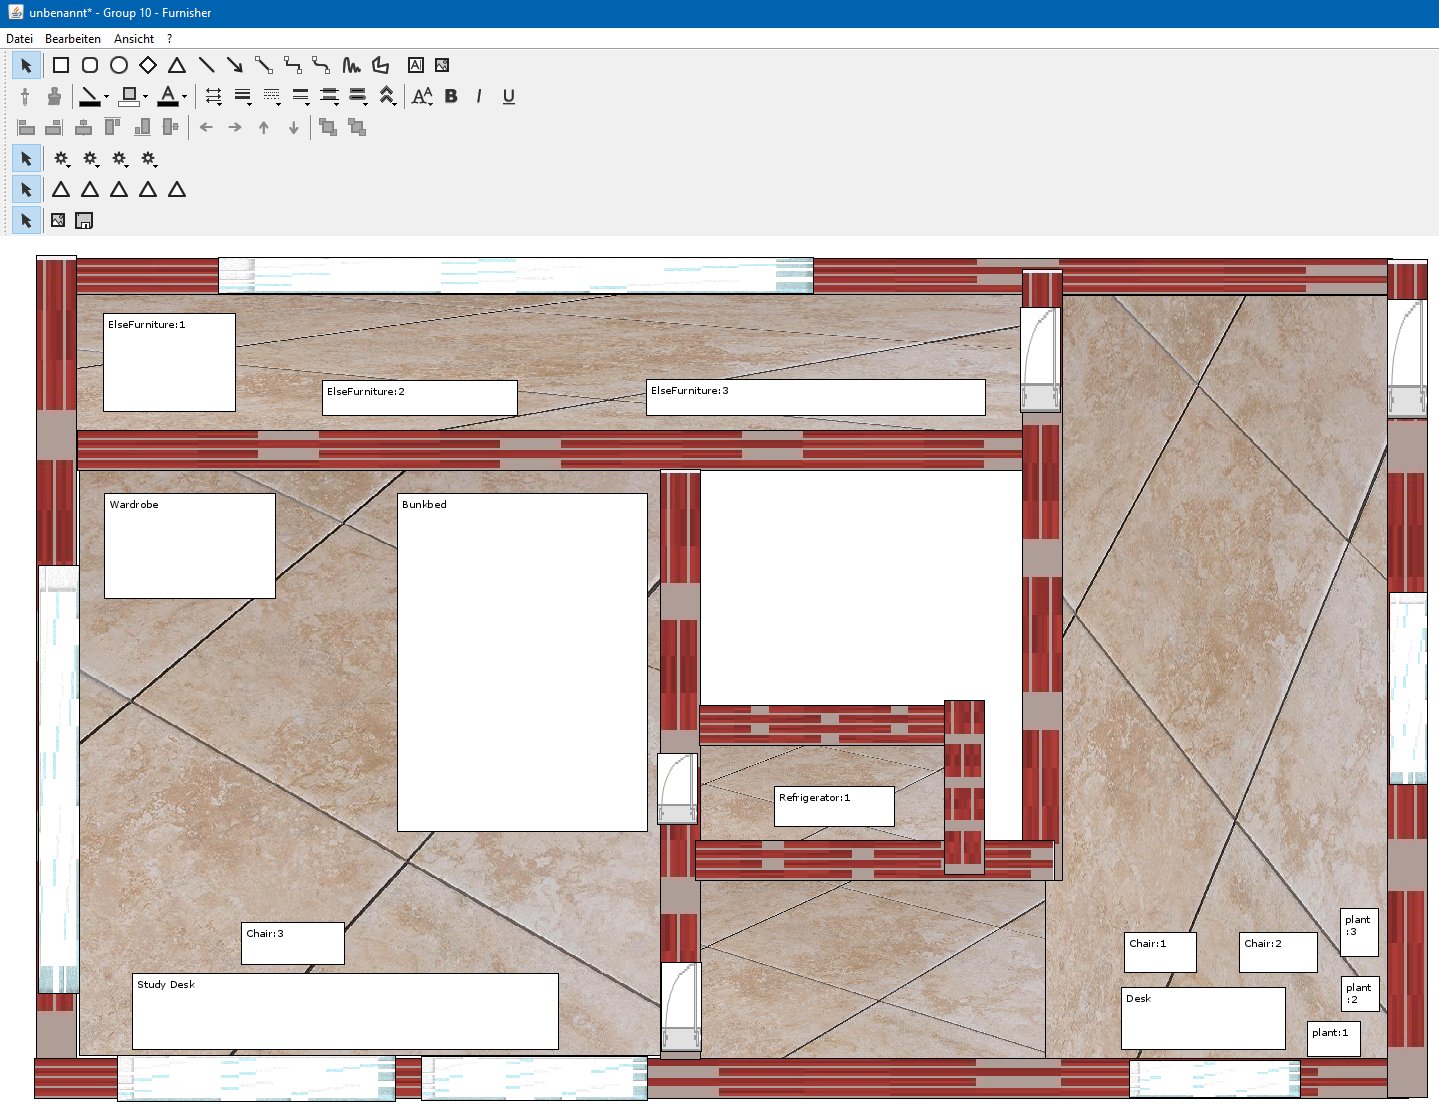
\includegraphics[keepaspectratio,width=\textwidth]{images/program.PNG}
	\caption{Organizing Furnitures on the Floorplan}
\end{figure}

\begin{figure}[h]
	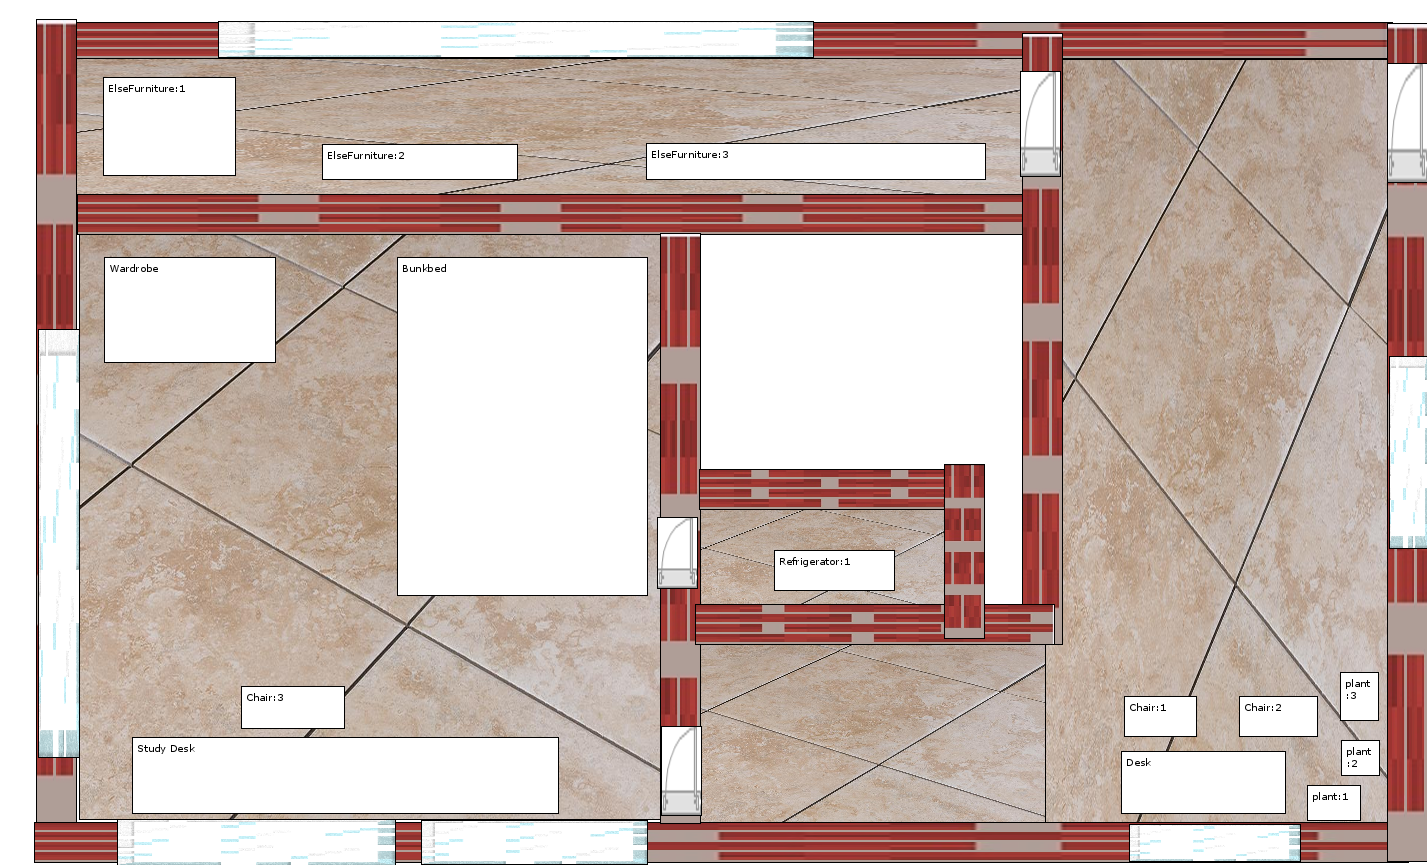
\includegraphics[keepaspectratio,width=\textwidth]{images/output.png}
	\caption{Exported Image}
\end{figure}


\end{document}